\chapter{Basic Theory Of Interest}

\refb{Further Reading}{
    D.G. Luenberger: Investment Science, Chapters 2,4
}

\section{Principal and Interest}
\egb{Interest}{If you invest \$1.00 in a bank account paying 8\% interest per year, at the end of the year, you will have \$1.08.}

\defb{Terminology}{
    \begin{itemize}
        \item \textbf{Principal}: The initial investment $(W)$.
        \item \textbf{Interest}: The rent paid on investment $(I)$.
        \item \textbf{Interest Rate}: Interest rate per unit of currency invested $(r)$.
        \item $\Rightarrow I = W \times r$
        \item \textbf{Initial Wealth (today)}: $W-0 = W$
        \item \textbf{Terminal Wealth (after one year)}: $W_1 = W(1+r)$
    \end{itemize}
}


\section{Compound Interest}
Consider a situation in which money is invested in a bank account over \textbf{several periods}. Assume that the \textbf{interest rate} in the \( n \)th year is \( r_n \) for \( n = 1, 2, 3, \ldots \). We obtain the following \textbf{account holdings}:
\begin{itemize}[label=\textbullet]
    \item today: \( W_0 = W \);
    \item after 1 year: \( W_1 = W(1 + r_1) \);
    \item after 2 years:
          \[
              W_2 = W_1(1 + r_2) = W(1 + r_1)(1 + r_2);
          \]
    \item after \( n \) years:
          \[
              W_n = W_{n-1}(1 + r_n) = W \prod_{i=1}^n (1 + r_i).
          \]
\end{itemize}

If the \textbf{interest rate is constant}, i.e., \( r_n = r \), then
\[
    W_n = W(1 + r)^n \quad \Rightarrow \quad r = \left( \frac{W_n}{W_0} \right)^{1/n} - 1.
\]

\begin{itemize}[label=\textbullet]
    \item The \textbf{seven-ten rule}:
          \begin{itemize}
              \item Money invested at \textbf{7\%} doubles in about \textbf{10 years};
              \item Money invested at \textbf{10\%} doubles in about \textbf{7 years} (Figure \ref{fig:compound_interest}).
          \end{itemize}
\end{itemize}

\begin{figure}[h!]
    \centering
    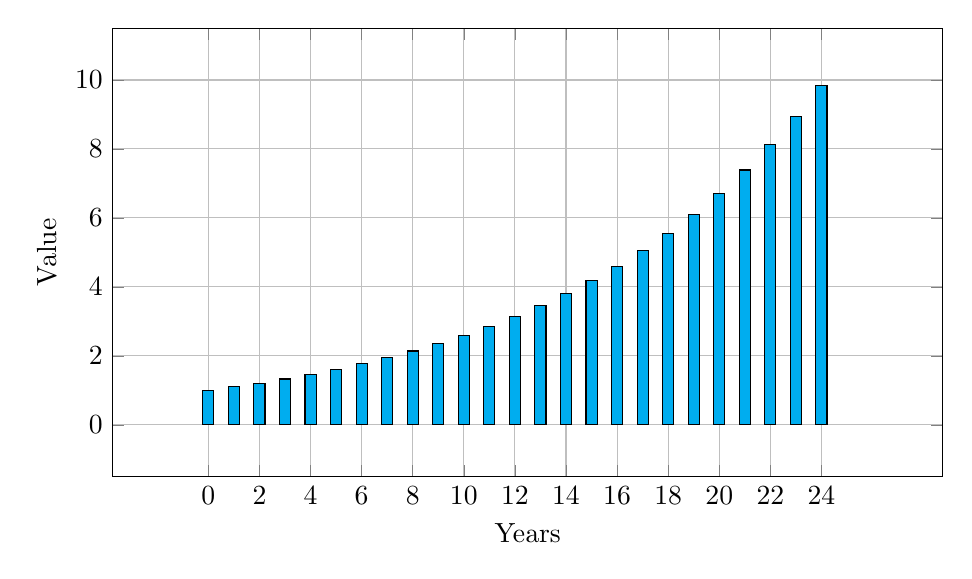
\begin{tikzpicture}
        \begin{axis}[
                width=\textwidth,
                height=0.6\textwidth,
                grid=major,
                xlabel={Years},
                ylabel={Value},
                ymin=0, ymax=10,
                xmin=0, xmax=25,
                ytick={0,2,4,6,8,10},
                xtick={0,2,...,24},
                legend pos=north west,
                bar width=4pt,
                enlargelimits=0.15,
                symbolic x coords={0, 1, 2, 3, 4, 5, 6, 7, 8, 9, 10, 11, 12, 13, 14, 15, 16, 17, 18, 19, 20, 21, 22, 23, 24, 25},
                ymajorgrids=true,
                xmajorgrids=true,
            ]
            \addplot[ybar,fill=cyan] plot coordinates {
                    (0,1) (1,1.10) (2,1.21) (3,1.33) (4,1.46) (5,1.61) (6,1.77) (7,1.95) (8,2.14) (9,2.36) (10,2.59)
                    (11,2.85) (12,3.14) (13,3.45) (14,3.80) (15,4.18) (16,4.60) (17,5.06) (18,5.56) (19,6.11) (20,6.72)
                    (21,7.39) (22,8.13) (23,8.94) (24,9.83)
                };
            % \legend{Value over time}
        \end{axis}
    \end{tikzpicture}
    \caption{Money doubling over time with compound interest.}
    \label{fig:compound_interest}
\end{figure}









\section{Compunding at Various Intervals}
It is traditional to quote the interest rate on a yearly basis but adjust the proportion of that interest rate over each compounding period. Divide a year into $m$ equally-spaced compounding periods.
\begin{itemize}
    \item \textbf{Nominal Interest Rate (annual)}: r
    \item \textbf{Length of a compounding period} : \( \frac{1}{m} \) years
    \item \textbf{Interest Rate for each of the $m$ periods}: : \( r \frac{1}{m} \)
    \item \textbf{Growth of account over $k$ compounding periods}: \((1 + \frac{r}{m})^{k} \)
    \item \textbf{Growth of account over 1 year}: \((1 + \frac{r}{m})^{m} \)
    \item \textbf{The effective interest rate} is the number $r_{\text{eff}}$ such that \((1 + r_{\text{eff}})^{m} = (1 + \frac{r}{m})^{m}\)
\end{itemize}

\section{Continuous Compounding}
Notice that increasing the number of compounding periods $m$ to infinity gives us the exponential function. If we measure time in years as $t$, we have:

\begin{equation}
    \lim_{m \to \infty} \left(1 + \frac{r}{m}\right)^{mt} \rightarrow e^{rt}
\end{equation}


\begin{figure}[h!]
    \centering
    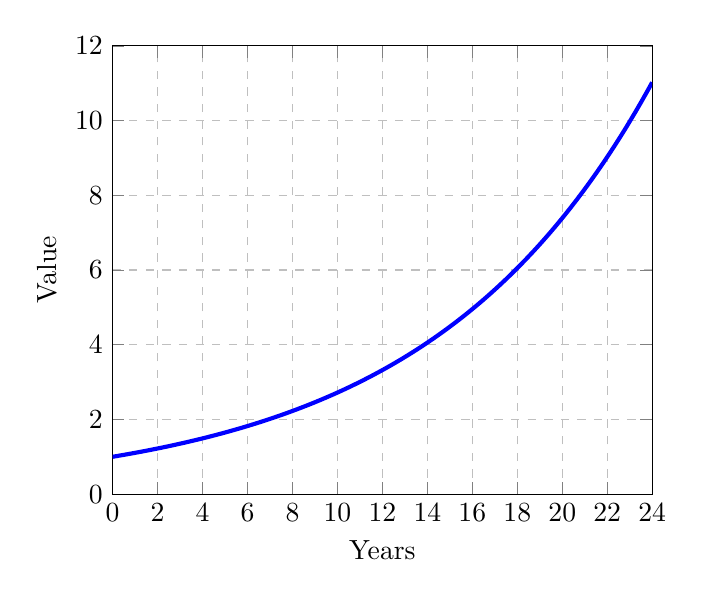
\begin{tikzpicture}
        \begin{axis}[
                xlabel={Years},
                ylabel={Value},
                xmin=0, xmax=24,
                ymin=0, ymax=12,
                xtick={0,2,4,6,8,10,12,14,16,18,20,22,24},
                ytick={0,2,4,6,8,10,12},
                grid=major,
                grid style=dashed,
                domain=0:24,
                samples=100,
            ]
            \addplot[
                color=blue,
                line width=1.5pt
            ]
            {exp(0.10*x)};
        \end{axis}
    \end{tikzpicture}
    \caption{Exponential growth. For continuous compounding at 10\% the value of \$1 doubles in about 7 years, and grows 8 times in about 20 years.}
\end{figure}

\section{Time Value of Money}
\defb{Debt}{
    Money has a time value, and is worth more in the present than the future. In other words, money invested/borrowed today leads to increased value/debt in the future as a result of interest. \bigskip

    If I make a deposit in the bank (meaning that I only need it in the future, not the present), it grows over time due to interest compounding. \bigskip

    Similarly, if I borrow from the bank at an interest rate $r$ (meaning I need money now that I can only pay it back in the future), my debt to the bank increases over time following the the compounding of interest.
}

\defb{Present Value}{
    Suppose that the annual interest rate $r$ is compounded $m$ times per year. \bigskip

    The final amount attained is denoted as $A$ which is in the future. This amount can also be equivalently represented as an amount $d_kA$ today, which is $A$ discounted to the present, where

    \[d_k = \frac{1}{(1+r/m)^{k}} < 1\]

    $d_k$ is the discount factor, and $d_kA$ is the present value of $A$.
}
\marginnote{A certificate of deposit is a promise for the bank to pay interest on money deposited for a fixed period. Banks generally compensate a longer lock-in period with higher interest rates. This is because a longer duration of lock-in period increases the unertainty regarding future interest rate movements and inflation. \\\bigskip


    For example, in a volatile period of time in the economy, locking-in a deposit at a fixed rate for 2 years might mean you could lose out on better rates if interest rates increase next year. But also, you could also keep a better rate if interest rates decrease next year.}
\vspace{-7pt}

\defb{The Ideal Bank}{
    An \textbf{ideal bank}, for the sake of modelling purposes:
    \begin{itemize}
        \item Applies the same interest rate to deposits and limitations
        \item Assumes no additional service charges or transaction customizations
        \item Has a constant interest rate regardless of the size of principal (amount of money loaned or deposited)
    \end{itemize} \bigskip

    In practice, different transactions may have different rates based on their duration. For example, a 2-year certificate of deposit (CD) might offer a higher rate than a 1-year CD. \bigskip

    A \textbf{constant ideal bank} has a constant interest rate that is indepedent of duration.
}

\section{Future and Present Value of Streams}

\begin{itemize}
    \item Consider a \textbf{cash flow stream} \( x_0, x_1, x_2, \ldots, x_n \).
    \item \( x_k \) occurs at the end of period \( k \).
    \item We can use a \textbf{constant ideal bank} to move all cash flows to the end of period \( n \) or to the \textbf{present time}.
\end{itemize}

\defb{Future Value}{
    The \textbf{future value} of the stream is
    \[
        \text{FV} = \sum_{k=0}^{n} x_k (1 + r/m)^{n-k} \quad \leftarrow \text{`compounding'}
    \]
}

\defb{Present Value}{
    The \textbf{present value} of the stream is
    \[
        \text{PV} = \sum_{k=0}^{n} \frac{x_k}{(1 + r/m)^{k}} \quad \leftarrow \text{`discounting'}
    \]
}

\begin{figure}[h!]
    \centering
    \begin{tikzpicture}[>=Stealth, scale=0.6]
    
    % First diagram (compounding)
    \begin{scope}
        \draw[->] (0,0) -- (7,0) node[right] {time};
        \node at (0,0) {$\bullet$};
        \draw[->] (0,0) -- (0,-1) node[below] {$x_0$};
        \draw[->] (1,0) -- (1,1) node[above] {$x_1$};
        \draw[->] (2,0) -- (2,2) node[above] {$x_2$};
        \draw[->] (3,0) -- (3,-1) node[below] {$x_3$};
        \draw[->] (4,0) -- (4,1) node[above] {$x_4$};
        \draw[->] (5,0) -- (5,2) node[above] {$x_5$};
        \draw[->] (6,0) -- (6,1.5) node[above] {$x_6$};
        \node[align=center] at (10.5,0) {compounding \\ \textcolor{red}{$\rightarrow$}};

        \draw[->] (13,0) -- (20,0) node[right] {time};
        \node at (13,0) {$\bullet$};
        \draw[->] (19,0) -- (19,2.5) node[above] {FV};
    \end{scope}
    
    % Second diagram (discounting)
    \begin{scope}[yshift=-4cm]
        \draw[->] (0,0) -- (7,0) node[right] {time};
        \node at (0,0) {$\bullet$};
        \draw[->] (0,0) -- (0,-1) node[below] {$x_0$};
        \draw[->] (1,0) -- (1,1) node[above] {$x_1$};
        \draw[->] (2,0) -- (2,2) node[above] {$x_2$};
        \draw[->] (3,0) -- (3,-1) node[below] {$x_3$};
        \draw[->] (4,0) -- (4,1) node[above] {$x_4$};
        \draw[->] (5,0) -- (5,2) node[above] {$x_5$};
        \draw[->] (6,0) -- (6,1.5) node[above] {$x_6$};
        \node[align=center] at (10.5,0) {discounting \\ \textcolor{red}{$\rightarrow$}};

        \draw[->] (13,0) -- (20,0) node[right] {time};
        \node at (13,0) {$\bullet$};
        \draw[->] (13,0) -- (13,2) node[above] {PV};
    \end{scope}
    
    \end{tikzpicture}
    \end{figure}


\section{Present Value and an Ideal Bank}
\debf{Equivalence of Streams}{
    Two cash flow streams are equivalent if they can be transofrmed into each other by an ideal bank.
}

\egb{
An ideal bank example
}{
    A bank with a 10\% interest rate could change a cash flow of $(1,0,0)$ to $(0,0,1.21)$ by receiving a deposit of $\$1 now and paying principal and interest of \$
}